\subsection{Desarrollo de la idea.}

\vspace*{0.3cm}

GRASP (Greedy Randomized Adaptative Search Procedure) es una combinación entre una heurística golosa ``aleatorizada'' y un procedimiento de búsqueda local.  La idea es la siguiente:

\begin{codebox}
\li \While no se alcance el {\it criterio de terminación}
\li \Do 
		Obtener una solución inicial mediante una {\it heurística golosa aleatorizada}.
\li 		Mejorar la solución mediante búsqueda local.
\li 		Recordar la mejor solución obtenida hasta el momento.
	\End
\end{codebox}

Como criterios de terminación, analizaremos dos casos particulares:

\begin{itemize}
\item Se realizaron $50$ iteraciones.
\item Se realizaron $10$ iteraciones sin encontrar una solución mejor.
\end{itemize}

En cuanto a la heurística golosa aleatorizada, hemos continuado con la idea del algoritmo goloso descrito anteriormente, con la variación de que, en cada paso, se genera una Lista Restricta de Candidatos (RCL) y se elige aleatoriamente un candidato de esa lista.  Analizaremos dos posibles maneras de construir dicha RCL:

\begin{enumerate}
\item Hallar al mejor candidato, es decir, el nodo que hemos definido como óptimo, y colocar en la RCL los nodos candidatos cuya cantidad de vecinos ``libres'' sea no menor a un $10 \%$ de la cantidad de vecinos ``libres'' del mejor candidato.
\item Hallar al mejor candidato y colocar en la RCL los $5$ mejores candidatos, es decir, los $5$ nodos que más nodos ``libres'' cubran.
\end{enumerate}

\vspace*{0.6cm}

\newpage
\subsection{Experimentación y gráficos.}

\vspace*{0.3cm}

En esta sección trataremos de encontrar, entre las posibles combinaciones de criterios de parada y listas restrictas de candidatos explicadas anteriormente, aquella que tenga el mejor balance entre calidad de solución y performance. Se ha elegido utilizar la segunda vecindad explicada en la sección de busqueda local, debido a su balance entre tiempo de ejecución y solución obtenida.  

Para facilitar la lectura, nombraremos a cada configuracón de la siguiente manera:

\begin{itemize}
	\item {\bf Configuración 1:} Utiliza como como criterio de parada realizar 10 iteraciones sin mejoras, y el primer RCL .
	\item {\bf Configuración 2:} Utiliza como como criterio de parada realizar 10 iteraciones sin mejoras, y el segundo RCL .
	\item {\bf Configuración 3:} Utiliza como como criterio de parada realizar 50 iteraciones, y el primer RCL .
	\item {\bf Configuración 4:} Utiliza como como criterio de parada realizar 50 iteraciones, y el segundo RCL .

\end{itemize}

Plantearemos entonces, experimentos que nos permitan observar cómo se desenvuelve nuestro algoritmo con cada configuración, y con los resultados, tratar de elegir una de ellas. Para ello se ha decidido evaluar instancias de tipo $circuito$, $estrella$, $galaxia$ y $aleatorio$.
 
\subsubsection{Circuitos}

Se generaron 20 $circuitos$ con entre 10 y 30 nodos.  El orden de los nodos fue aleatorizado para no depender de un rotulado en particular.

\paragraph{Performance} 

El gráfico obtenido con las mediciones de tiempo es el que se muestra en la Figura \ref{fig:4A}.

\begin{figure}[htb]
	\begin{center}
    		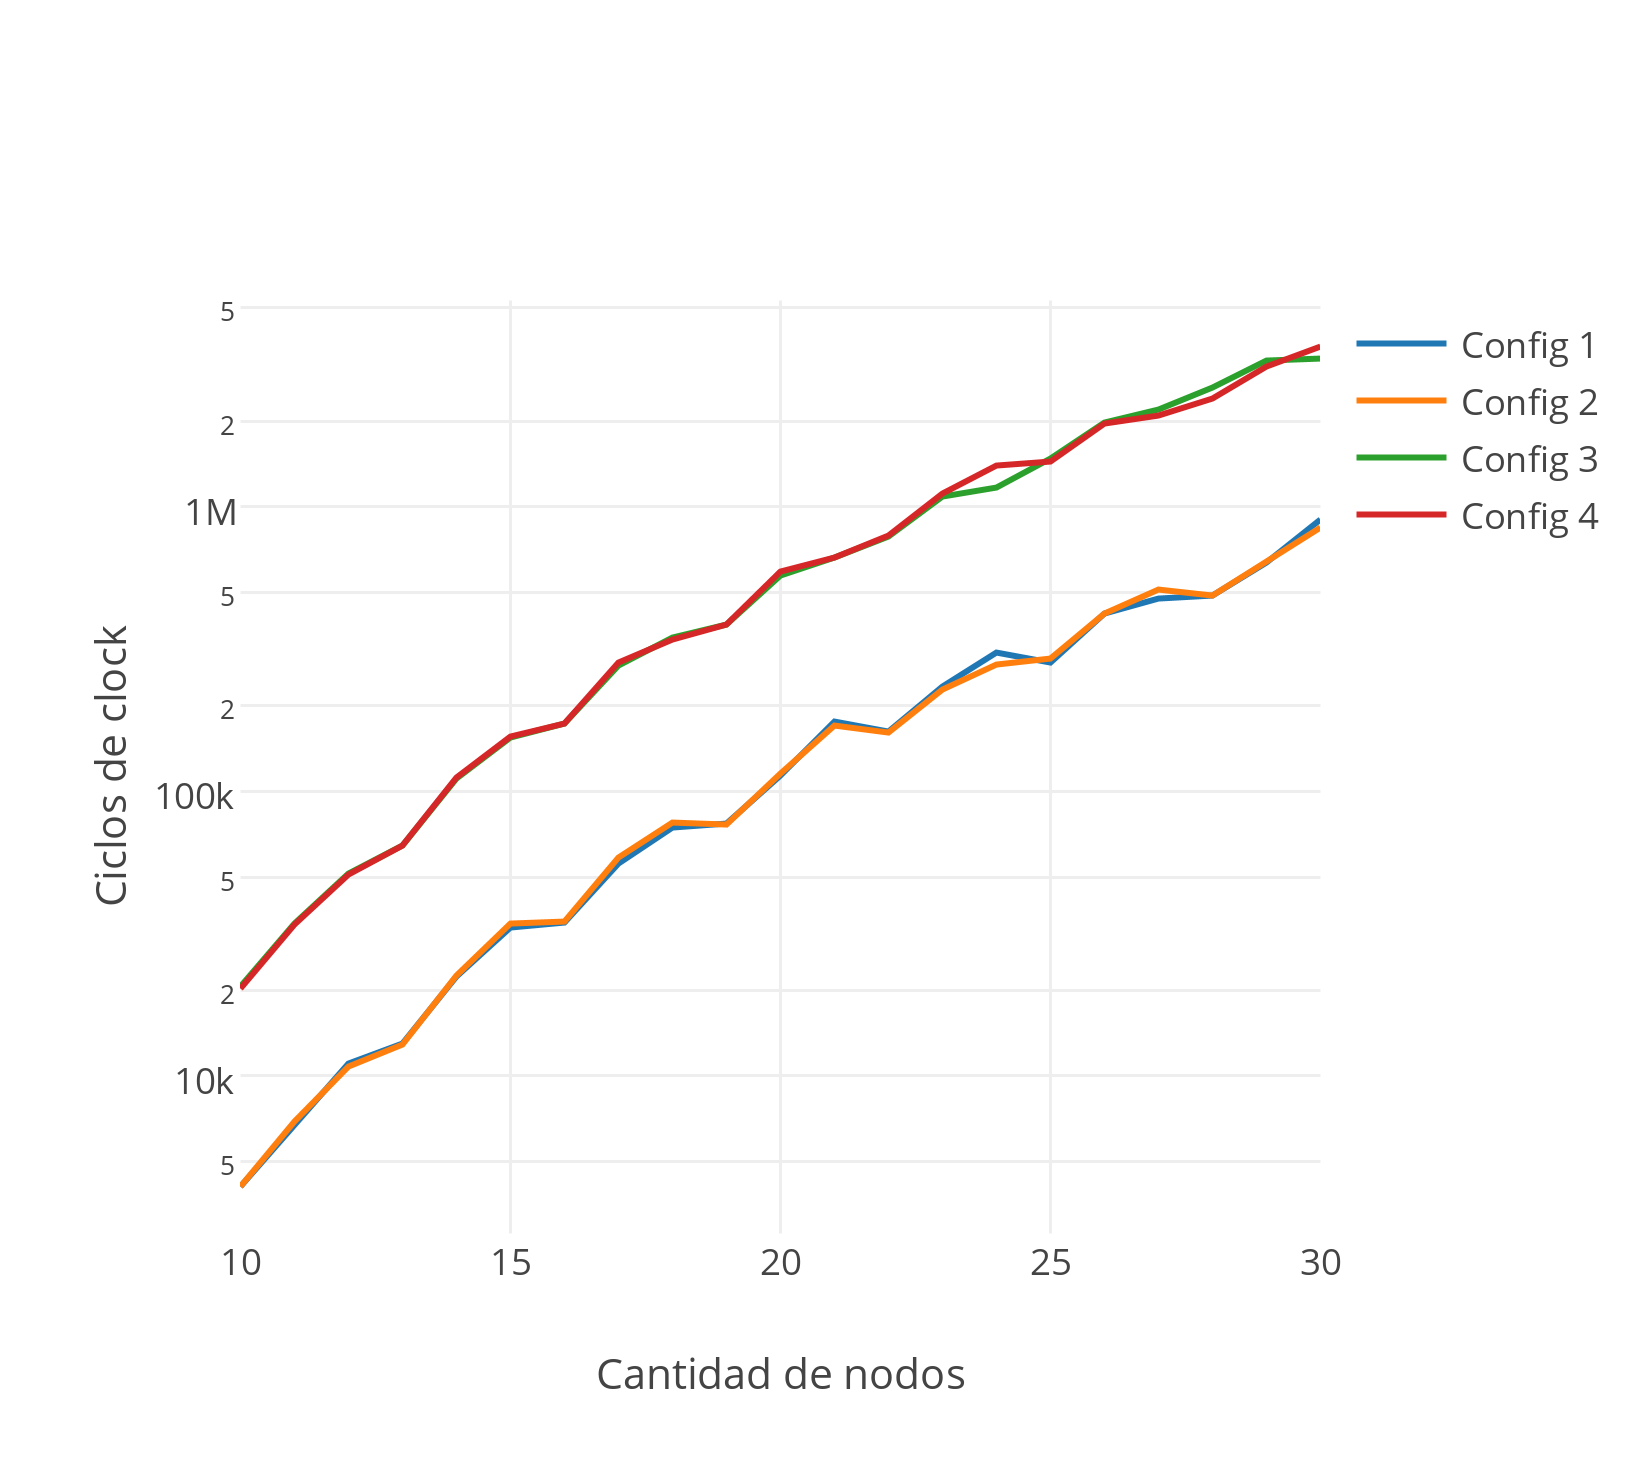
\includegraphics[scale=0.8]{imagenes/grasp-circuitos-tiempo.png}
	\end{center}
	\caption{GRASP - Circuitos}\label{fig:4A}
\end{figure}
%\FloatBarrier

La Figura parece indicar que aquellas configuraciones que utilizan el criterio de parada de 50 iteraciones(desde ahora llamado segundo criterio) tienen un desempeño peor que aquellas que utilizan el criterio de parada de 10 iteraciones sin mejora(desde ahora llamado primer criterio). Entre las configuraciones que utilizan el mismo criterio de parada, no parece ser posible indicar de manera precisa cual RCL optimiza más el tiempo de corrida del algoritmo.

\paragraph{Calidad} Se ha comparado el tamaño de la solución hallada con el tamaño de la solución exacta.  Los porcentajes de desaciertos sobre el total de instancias evaluadas son los siguientes:

\begin{verbatim}
Configuración 1: 0%
Configuración 2: 0%
Configuración 3: 0%
Configuración 4: 0%
\end{verbatim}

Pareciera entonces, que sin importar la configuración, para este tipo de grafos GRASP no provoca errores.
\subsubsection{Estrellas}

Se generaron 30 grafos $estrellas$ con grado máximo entre 5 y 7.

\paragraph{Performance}

La Figura \ref{fig:4B} muestra los resultados obtenidos respecto al tiempo de ejecución. Nuevamente, las configuraciones que utilizan el primer criterio de parada muestran un desempeño considerablemente mejor en términos de performance que aquellas que utilizan el segundo.
Se puede destacar, que la configuración 1 tiene el menor tiempo de ejecución.

\begin{figure}[htb]
	\begin{center}
    		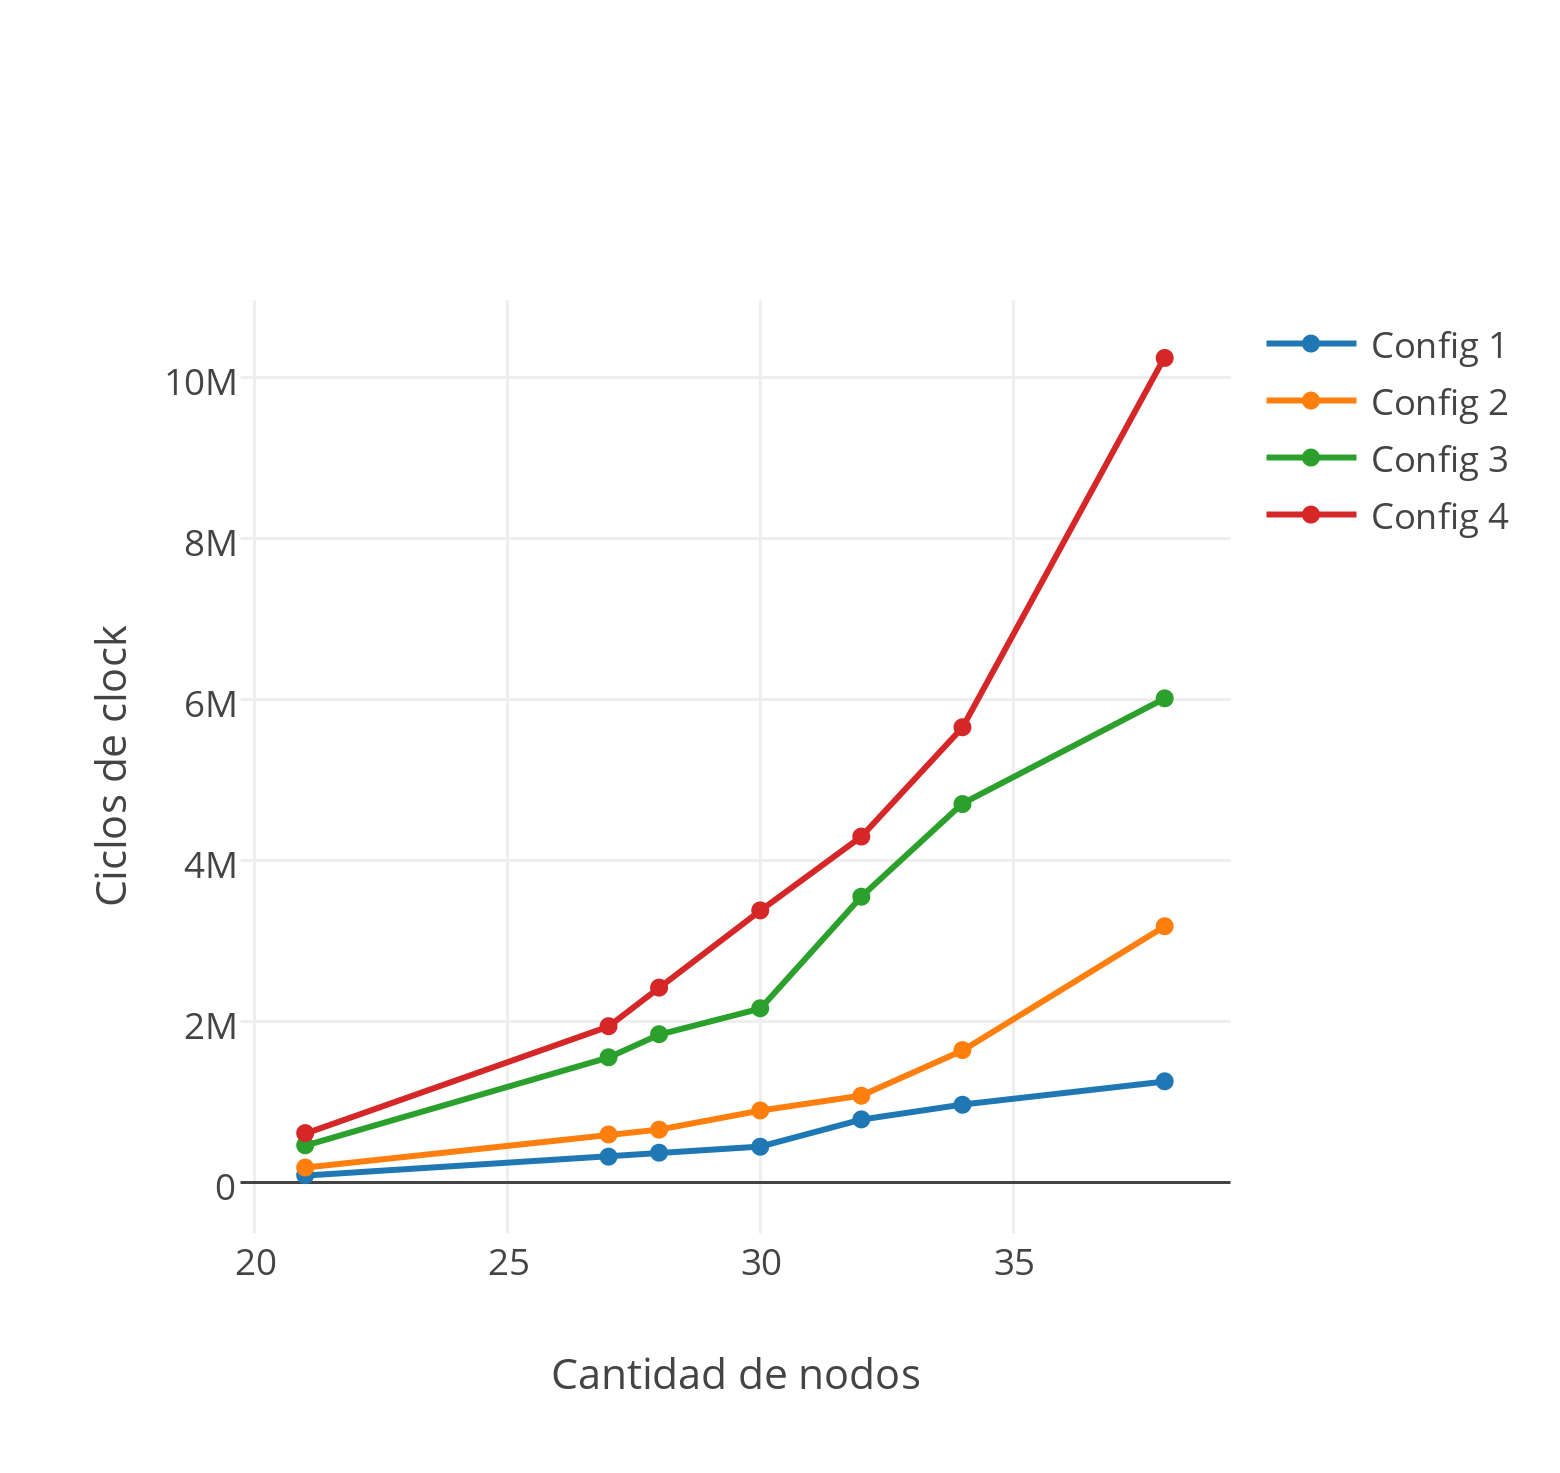
\includegraphics[scale=0.8]{imagenes/grasp-estrellas-tiempo.png}
	\end{center}
	\caption{GRASP - Estrellas}\label{fig:4B}
\end{figure}
%\FloatBarrier

\paragraph{Calidad} Se ha comparado el tamaño de la solución obtenida con el tamaño de la solución exacta. Los porcentajes de desaciertos sobre el total de instancias evaluadas son los siguientes:

\begin{verbatim}
Configuración 1: 3.34%
Configuración 2: 63.34%
Configuración 3: 0%
Configuración 4: 13.34%
\end{verbatim}

Podemos observar como la configuración 1 y 3 tienen las mejores tasas de acierto, llegando esta última a no cometer errores. Cabe destacar que la configuración 2 tiene para este tipo de grafos, un porcentaje de desaciertos muy amplio.

\subsubsection{Galaxias}

Se generaron 20 grafos $galaxia$ con entre 7 y 38 nodos.

\paragraph{Performance}

La Figura \ref{fig:4C} muestra los resultados obtenidos respecto al tiempo de ejecución. Aquí, las configuracion 1 es claramente la de mejor performance mientras que la 4 es claramente la de peor tiempo de ejecución. A priori, no podemos determinar según este gráfico quien tiene un mejor desempeño entre las configuraciones 2 y 3. 

\begin{figure}[htb]
	\begin{center}
    		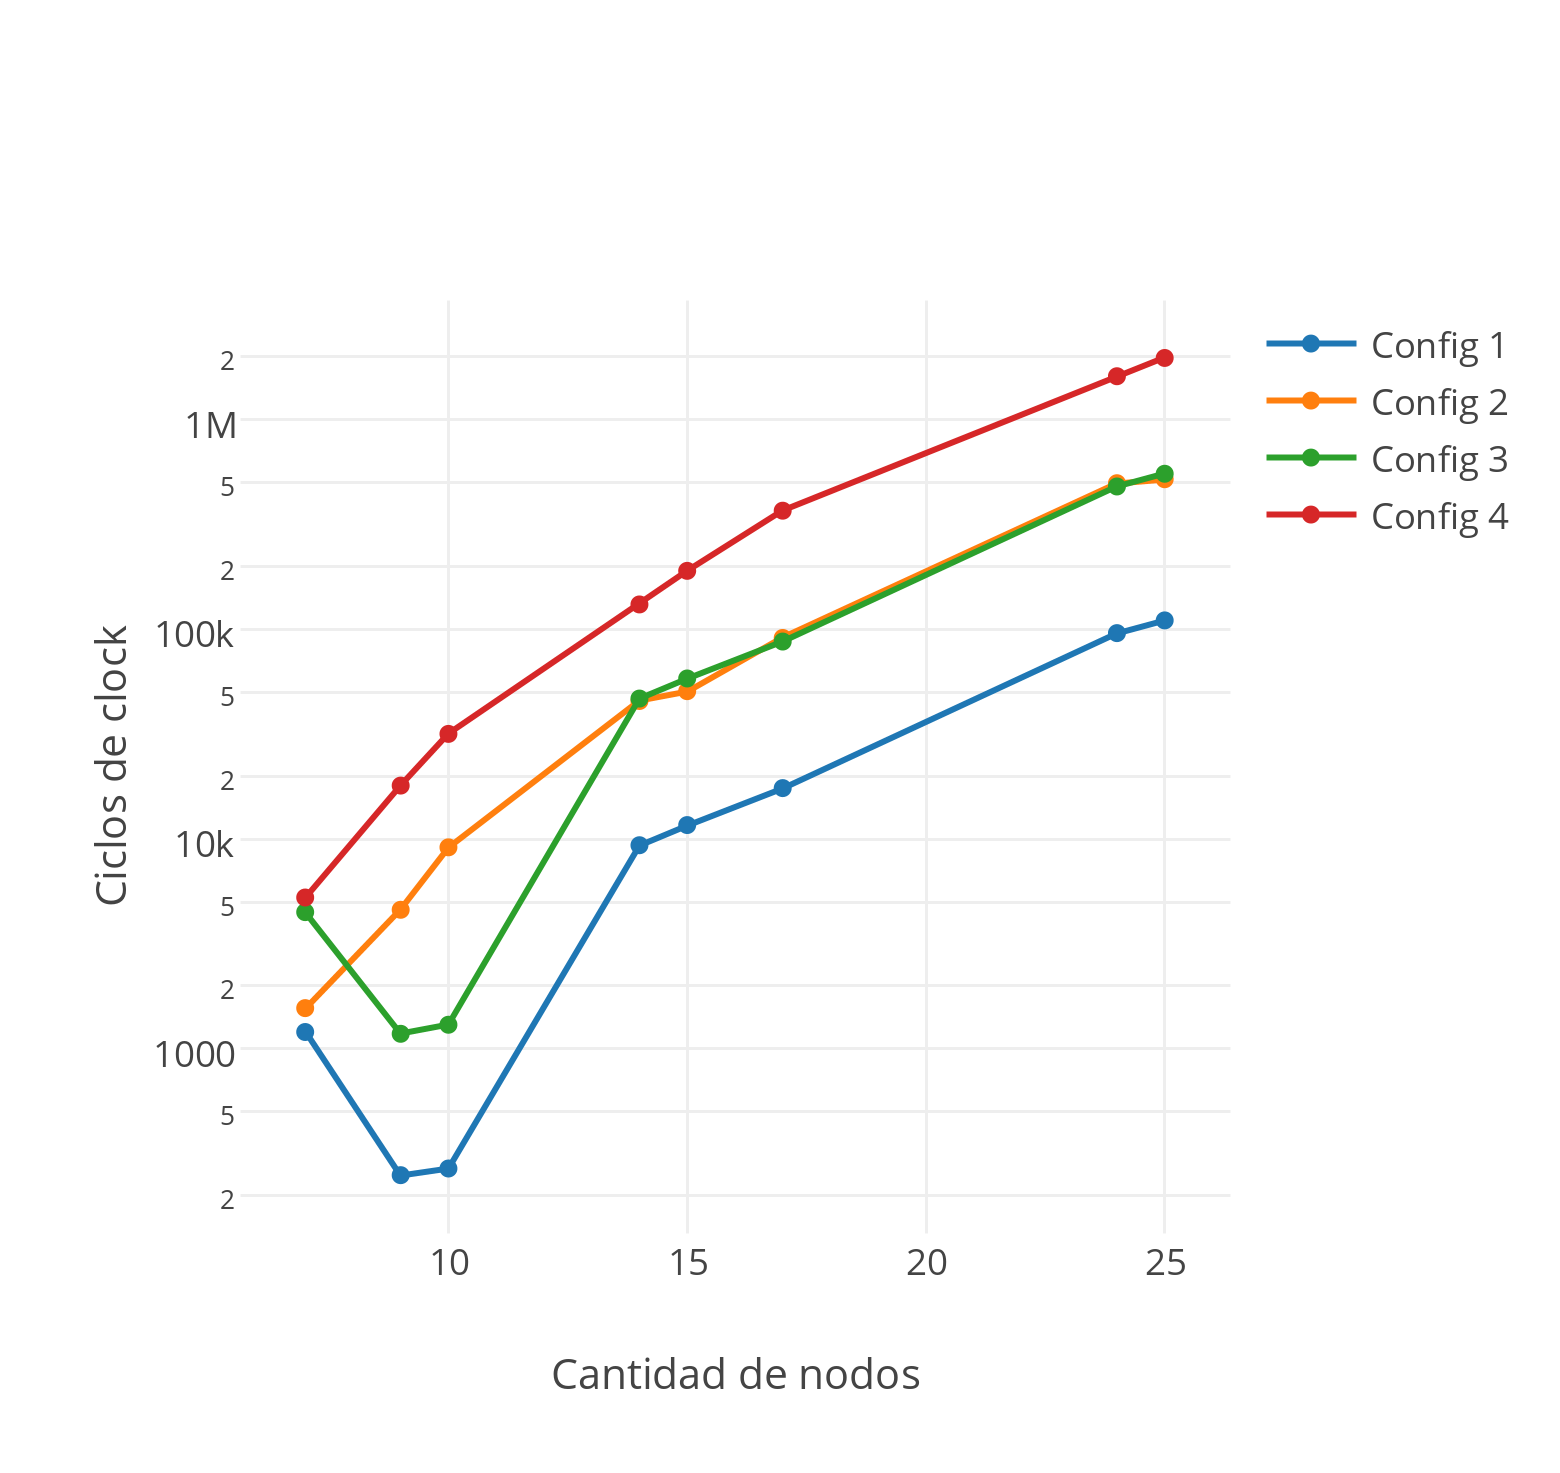
\includegraphics[scale=0.8]{imagenes/grasp-galaxias-tiempos.png}
	\end{center}
	\caption{GRASP - Galaxias}\label{fig:4C}
\end{figure}
%\FloatBarrier

\paragraph{Calidad} 
Se ha comparado el tamaño de la solución obtenida con el tamaño de la solución exacta. Los porcentajes de desaciertos sobre el total de instancias evaluadas son los siguientes:

\begin{verbatim}
Configuración 1: 0%
Configuración 2: 50%
Configuración 3: 0%
Configuración 4: 10%
\end{verbatim}

Podemos observar como las configuraciones 1 y 3 no tuvieron errores, como la configuración 4 vuelve a tener un error aceptable, y como la configuración 2 vuelve a tener una tasa de aciertos muy baja

\subsubsection{Aleatorios}

Para estos experimentos se han generado dos sets de instancias $aleatorias$. Uno contiene 120 grafos de entre 4 y 15 nodos, para poder contrastar con el algoritmo exacto (sólo se utilizara para la parte de calidad). El otro contiene 210 grafos de entre 10 y 30 nodos, que si bien no serán comparadas con el algoritmo exacto, posibilitará apreciar los tiempos de ejecución más ampliamente y tener una idea más general respecto a la calidad de las soluciones obtenidas.

\paragraph{Performance} La Figura \ref{fig:4D} muestra los resultados obtenidos respecto al tiempo de ejecución. Podemos apreciar que las configuraciones que utilizan el primer criterio de parada tienen un desempeño peor que las otras, y entre las configuraciones que utilizan el segundo criterio, la configuración 1 parecería mostrarse como la más óptima.

\begin{figure}[htb]
	\begin{center}
    		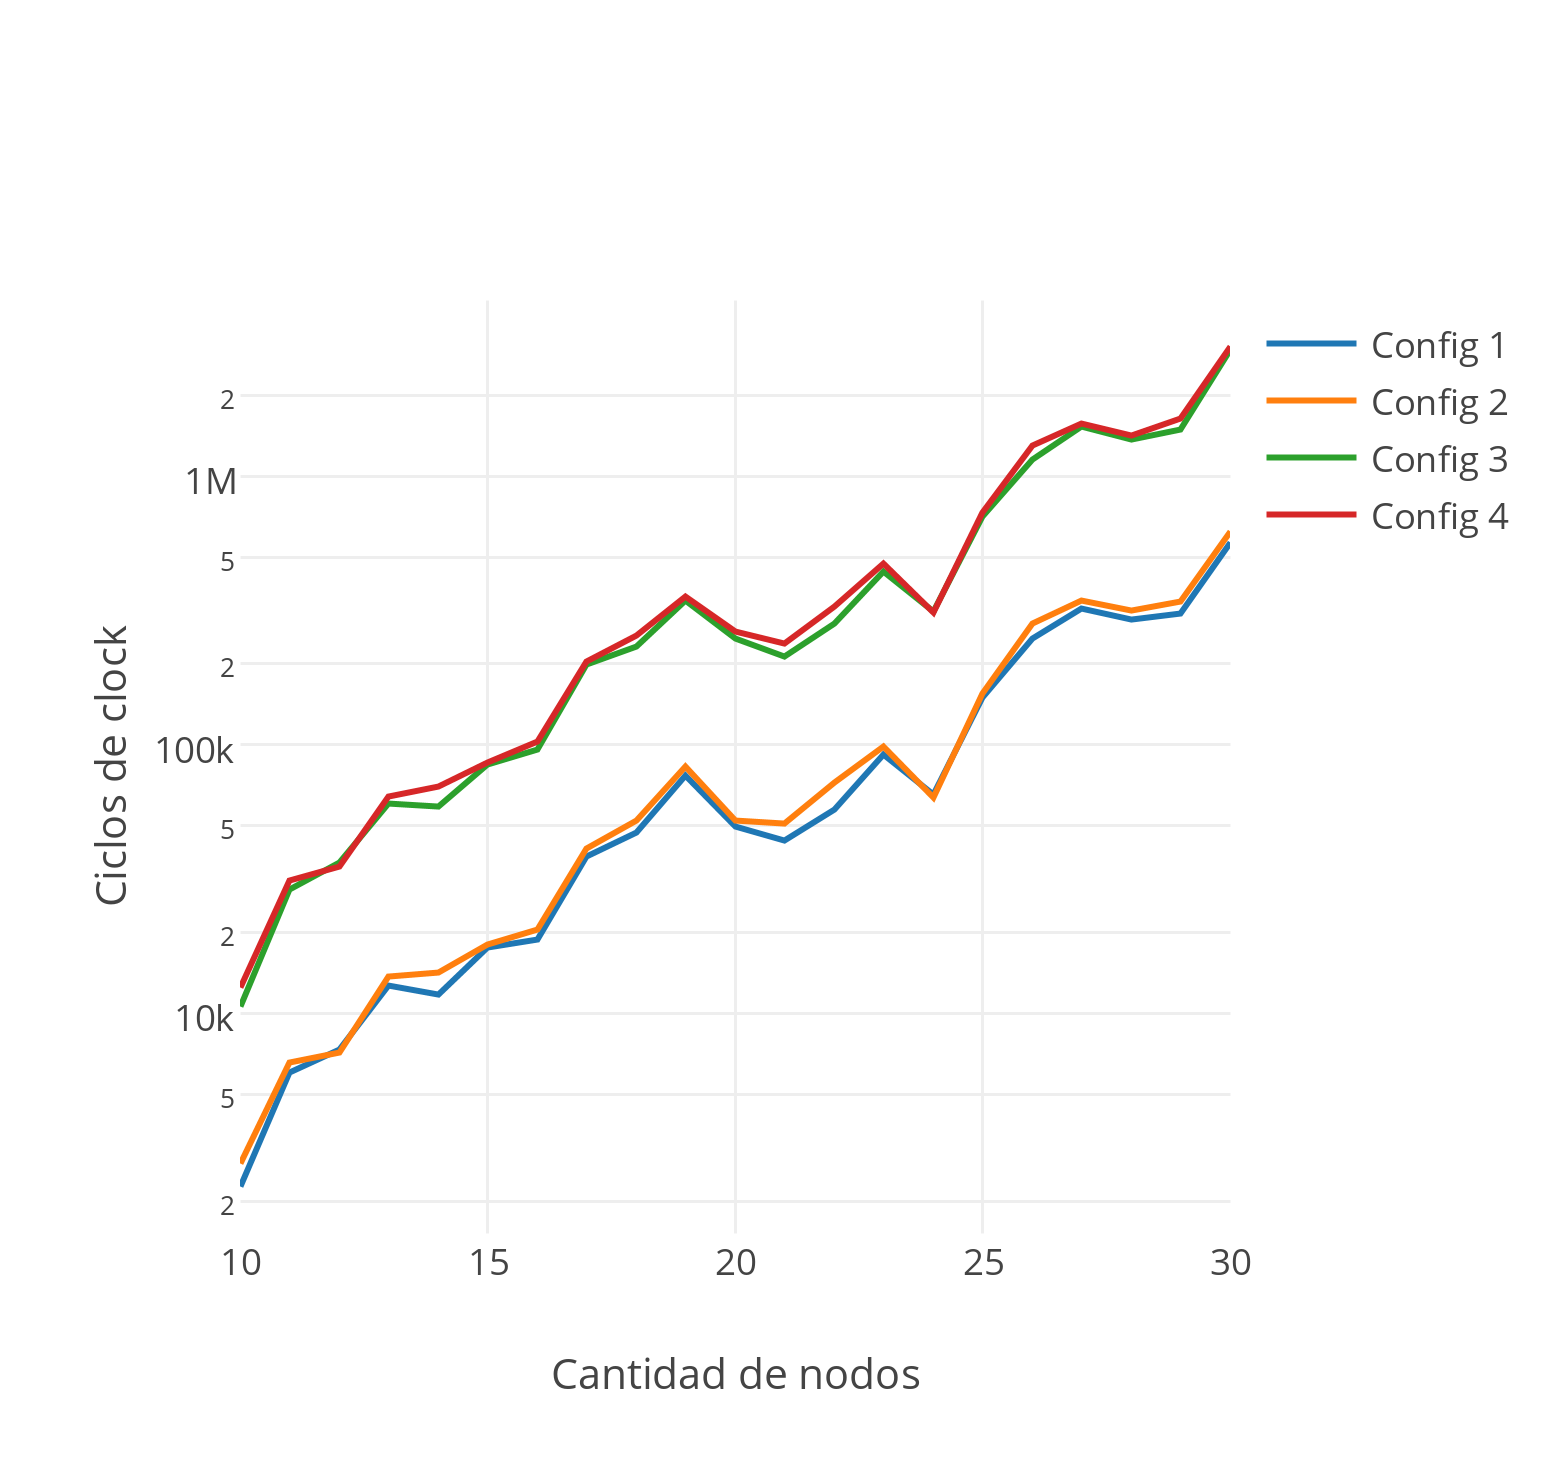
\includegraphics[scale=0.8]{imagenes/grasp-aleatorios-tiempo.png}
	\end{center}
	\caption{GRASP - Aleatorios}\label{fig:4D}
\end{figure}
%\FloatBarrier

\paragraph{Calidad} 

\subparagraph{Set 1} Se ha comparado el tamaño de la solución obtenida con el tamaño de la solución exacta.  Los porcentajes de desaciertos sobre el total de instancias evaluadas son los siguientes:

\begin{verbatim}
Configuración 1: 1.667%
Configuración 2: 0.833%
Configuración 3: 0%
Configuración 4: 0%
\end{verbatim}

Podemos observar que todas las configuraciones tienen una tasa de error muy baja, destacando la 3 y 4 que no tienen errores.

\subparagraph{Set 2} Como por el tamaño de estas instancias se dificulta la comparación con el algoritmo exacto, se consideró como la solución ``óptima'' en cada caso el menor valor obtenido entre las cuatro configuraciones, y se registró, para cada una, la cantidad de instancias en las que no se logró dicho valor. Los porcentajes de estos ``desaciertos'' sobre el total de instancias evaluadas son los siguientes:

\begin{verbatim}
Configuración 1: 1.90%
Configuración 2: 1.43%
Configuración 3: 0.48%
Configuración 4: 0.48%
\end{verbatim}

Podemos notar nuevamente como en el set 1, tasas de error muy bajas, destacando que las configuraciones 3 y 4 ahora tienen algún error.

\subsubsection{Conclusiones} 

Luego de realizar este análisis para distintas instancias, podemos observar que, en lo que respecta a la calidad de las soluciones obtenidas, la configuracion 3 es la que logra obtener mejores resultados. Cabe destacar que si bien para las familias analizadas la configuración 2 arrojo muchos desaciertos, para casos generales esto no sucede. Por otro lado, las configuraciones que utilizan el segundo criterio, requieren un tiempo de ejecución considerablemente mayor que aquellas que utilizan el primero.  Por este motivo, si bien la Configuración 3 es la que se muestra mejor en calidad, decidimos considerar a la Configuración 1 como la que mejor balancea calidad y performance. Notece, que si bien la configuración 2 tiene mejor calidad para aleatorios, configuración 1 no tiene calidad mucho peor para estos casos, tiene una considerable mejor calidad para las familias estudiadas, y es ligeramente más optimo en tiempo.